%\VignetteIndexEntry{Introduction to the dataRetrieval package}
%\VignetteEngine{knitr::knitr}
%\VignetteDepends{}
%\VignetteSuggests{xtable,EGRET}
%\VignetteImports{zoo, XML, RCurl}
%\VignettePackage{dataRetrieval}

\documentclass[a4paper,11pt]{article}\usepackage{graphicx, color}
%% maxwidth is the original width if it is less than linewidth
%% otherwise use linewidth (to make sure the graphics do not exceed the margin)
\makeatletter
\def\maxwidth{ %
  \ifdim\Gin@nat@width>\linewidth
    \linewidth
  \else
    \Gin@nat@width
  \fi
}
\makeatother

\definecolor{fgcolor}{rgb}{0.2, 0.2, 0.2}
\newcommand{\hlnumber}[1]{\textcolor[rgb]{0,0,0}{#1}}%
\newcommand{\hlfunctioncall}[1]{\textcolor[rgb]{0.501960784313725,0,0.329411764705882}{\textbf{#1}}}%
\newcommand{\hlstring}[1]{\textcolor[rgb]{0.6,0.6,1}{#1}}%
\newcommand{\hlkeyword}[1]{\textcolor[rgb]{0,0,0}{\textbf{#1}}}%
\newcommand{\hlargument}[1]{\textcolor[rgb]{0.690196078431373,0.250980392156863,0.0196078431372549}{#1}}%
\newcommand{\hlcomment}[1]{\textcolor[rgb]{0.180392156862745,0.6,0.341176470588235}{#1}}%
\newcommand{\hlroxygencomment}[1]{\textcolor[rgb]{0.43921568627451,0.47843137254902,0.701960784313725}{#1}}%
\newcommand{\hlformalargs}[1]{\textcolor[rgb]{0.690196078431373,0.250980392156863,0.0196078431372549}{#1}}%
\newcommand{\hleqformalargs}[1]{\textcolor[rgb]{0.690196078431373,0.250980392156863,0.0196078431372549}{#1}}%
\newcommand{\hlassignement}[1]{\textcolor[rgb]{0,0,0}{\textbf{#1}}}%
\newcommand{\hlpackage}[1]{\textcolor[rgb]{0.588235294117647,0.709803921568627,0.145098039215686}{#1}}%
\newcommand{\hlslot}[1]{\textit{#1}}%
\newcommand{\hlsymbol}[1]{\textcolor[rgb]{0,0,0}{#1}}%
\newcommand{\hlprompt}[1]{\textcolor[rgb]{0.2,0.2,0.2}{#1}}%

\usepackage{framed}
\makeatletter
\newenvironment{kframe}{%
 \def\at@end@of@kframe{}%
 \ifinner\ifhmode%
  \def\at@end@of@kframe{\end{minipage}}%
  \begin{minipage}{\columnwidth}%
 \fi\fi%
 \def\FrameCommand##1{\hskip\@totalleftmargin \hskip-\fboxsep
 \colorbox{shadecolor}{##1}\hskip-\fboxsep
     % There is no \\@totalrightmargin, so:
     \hskip-\linewidth \hskip-\@totalleftmargin \hskip\columnwidth}%
 \MakeFramed {\advance\hsize-\width
   \@totalleftmargin\z@ \linewidth\hsize
   \@setminipage}}%
 {\par\unskip\endMakeFramed%
 \at@end@of@kframe}
\makeatother

\definecolor{shadecolor}{rgb}{.97, .97, .97}
\definecolor{messagecolor}{rgb}{0, 0, 0}
\definecolor{warningcolor}{rgb}{1, 0, 1}
\definecolor{errorcolor}{rgb}{1, 0, 0}
\newenvironment{knitrout}{}{} % an empty environment to be redefined in TeX

\usepackage{alltt}

\usepackage{amsmath}
\usepackage{times}
\usepackage{hyperref}
\usepackage[numbers, round]{natbib}
\usepackage[american]{babel}
\usepackage{authblk}
\usepackage{subfig}
\usepackage{placeins}
\usepackage{footnote}
\usepackage{tabularx}
\renewcommand\Affilfont{\itshape\small}

\renewcommand{\topfraction}{0.85}
\renewcommand{\textfraction}{0.1}
\usepackage{graphicx}


\textwidth=6.2in
\textheight=8.5in
\parskip=.3cm
\oddsidemargin=.1in
\evensidemargin=.1in
\headheight=-.3in

%------------------------------------------------------------
% newcommand
%------------------------------------------------------------
\newcommand{\scscst}{\scriptscriptstyle}
\newcommand{\scst}{\scriptstyle}
\newcommand{\Robject}[1]{{\texttt{#1}}}
\newcommand{\Rfunction}[1]{{\texttt{#1}}}
\newcommand{\Rclass}[1]{\textit{#1}}
\newcommand{\Rpackage}[1]{\textit{#1}}
\newcommand{\Rexpression}[1]{\texttt{#1}}
\newcommand{\Rmethod}[1]{{\texttt{#1}}}
\newcommand{\Rfunarg}[1]{{\texttt{#1}}}
\IfFileExists{upquote.sty}{\usepackage{upquote}}{}

\begin{document}






%------------------------------------------------------------
\title{The dataRetrieval R package}
%------------------------------------------------------------
\author[1]{Laura De Cicco}
\author[1]{Robert Hirsch}
\affil[1]{United States Geological Survey}






\maketitle
\tableofcontents

%------------------------------------------------------------
\section{Introduction to dataRetrieval}
%------------------------------------------------------------ 
The dataRetrieval package was created to simplify the process of getting hydrologic data in the R enviornment. It has been specifically designed to work seamlessly with the EGRET R package: Exploration and Graphics for RivEr Trends (EGRET). See: \url{https://github.com/USGS-R/EGRET/wiki} for information on EGRET. EGRET is designed to provide analysis of water quality data sets using the WRTDS method of data analysis (WRTDS is Weighted Regressions on Time, Discharge and Season) as well as analysis of discharge trends using robust time-series smoothing techniques.  Both of these capabilities provide both tabular and graphical analyses of long-term data sets.


The dataRetrieval package is designed to retrieve many of the major data types of USGS hydrologic data that are available on the web, but also allows users to make use of other data that they supply from spreadsheets.  Section 2 provides examples of how one can obtain raw data from USGS sources on the web and ingest them into data frames within the R environment.  The functionality described in section 2 is for general use and is not tailored for the specific uses of the EGRET package.  The functionality described in section 3 is tailored specifically to obtaining input from the web and structuring them specifically for use in the EGRET package.  The functionality described in section 4 is for converting hydrologic data from user-supplied spreadsheets and structuring them specifically for use in the EGRET package.

For information on getting started in R and installing the package, see Appendix (\ref{sec:appendix1}): Getting Started.


%------------------------------------------------------------
\section{General USGS Web Retrievals}
%------------------------------------------------------------ 
In this section, we will run through 5 examples, documenting how to get raw data from the web. This includes site information (\ref{sec:usgsSite}), measured parameter information (\ref{sec:usgsParams}), historical daily values(\ref{sec:usgsDaily}), real-time (unit) values (\ref{sec:usgsRT}), and water quality data (\ref{sec:usgsWQP}) or (\ref{sec:usgsSTORET}). We will use the Choptank River near Greensboro, MD as an example.  The site-ID for this gage station is 01491000. Daily discharge measurements are available as far back as 1948.  Additionally, forms of nitrate have been measured dating back to 1964. The functions/examples in this section are for raw data retrieval.  This may or may not be the easiest data to work with.  In the next section, we will use functions that retrieve and process the data in a dataframe that may prove more friendly for R analysis.

%------------------------------------------------------------
\subsection{Introduction}
%------------------------------------------------------------
The United States Geological Survey organizes their hydrological data in standard structure.  Streamgages are located throughout the United States, and each streamgage has a unique ID.  Often (but not always), these ID's are 8 digits.  The first step to finding data is discoving this 8-digit ID. There are many ways to do this, one is the National Water Information System: Mapper \url{http://maps.waterdata.usgs.gov/mapper/index.html}.

Once the site-ID is known, the next required input for USGS data retrievals is the 'parameter code'.  This is a 5-digit code that specifies what measured paramater is being requested.  A complete list of possible USGS parameter codes can be found at \url{http://go.usa.gov/bVDz}.

Not every station will measure all parameters. A short list of commonly measured parameters is shown in Table \ref{tab:params}.


% latex table generated in R 3.0.1 by xtable 1.7-1 package
% Thu Aug 01 16:23:09 2013
\begin{table}[ht]
\centering
\begin{tabular}{rll}
  \hline
 & pCode & shortName \\ 
  \hline
1 & 00060 & Discharge [cfs] \\ 
  2 & 00065 & Gage height [ft] \\ 
  3 & 00010 & Temperature [C] \\ 
  4 & 00045 & Precipitation [in] \\ 
  5 & 00400 & pH \\ 
   \hline
\end{tabular}
\caption{Common USGS Parameter Codes} 
\label{tab:params}
\end{table}



For real-time data, the parameter code and site ID will suffice.  For most variables that are measured on a continuous basis, the USGS stores the historical data as daily values.  These daily values may be in the form of statistics such as the daily mean values, but they can also include daily maximums, minimums or medians.  These different statistics are specified by a 5-digit \texttt{"}stat code\texttt{"}.  A complete list of stat codes can be found here:

\url{http://nwis.waterdata.usgs.gov/nwis/help/?read_file=stat&format=table}

Some common stat codes are shown in Table \ref{tab:stat}.
% latex table generated in R 3.0.1 by xtable 1.7-1 package
% Thu Aug 01 16:23:09 2013
\begin{table}[ht]
\centering
\begin{tabular}{rll}
  \hline
 & StatCode & shortName \\ 
  \hline
1 & 00001 & Maximum \\ 
  2 & 00002 & Minimum \\ 
  3 & 00003 & Mean \\ 
  4 & 00008 & Median \\ 
   \hline
\end{tabular}
\caption{Commonly used USGS Stat Codes} 
\label{tab:stat}
\end{table}



\FloatBarrier

%------------------------------------------------------------
\subsection{Site Information}
\label{sec:usgsSite}
%------------------------------------------------------------

%------------------------------------------------------------
\subsubsection{getSiteFileData}
\label{sec:usgsSiteFileData}
%------------------------------------------------------------
Use the getSiteFileData function to obtain all of the information available for a particular USGS site such as full station name, drainage area, latitude, and longitude:


\begin{knitrout}
\definecolor{shadecolor}{rgb}{0.969, 0.969, 0.969}\color{fgcolor}\begin{kframe}
\begin{alltt}
\hlfunctioncall{library}(dataRetrieval)
\hlcomment{# Site ID for Choptank River near Greensboro, MD}
siteNumber <- \hlstring{"01491000"} 
ChoptankInfo <- \hlfunctioncall{getSiteFileData}(siteNumber)
\end{alltt}
\end{kframe}
\end{knitrout}


A list of the available columns are found in Appendix \ref{sec:appendix2INFO}: INFO dataframe. Pulling out a specific example piece of information, in this case station name can be done as follows:

\begin{knitrout}
\definecolor{shadecolor}{rgb}{0.969, 0.969, 0.969}\color{fgcolor}\begin{kframe}
\begin{alltt}
ChoptankInfo$station.nm
\end{alltt}
\begin{verbatim}
[1] "CHOPTANK RIVER NEAR GREENSBORO, MD"
\end{verbatim}
\end{kframe}
\end{knitrout}

Site information is obtained from \url{http://waterservices.usgs.gov/rest/Site-Test-Tool.html}
\FloatBarrier

%------------------------------------------------------------
\subsubsection{getDataAvailability}
\label{sec:usgsDataAvailability}
%------------------------------------------------------------
To find out the available data at a particular USGS site, including measured parameters, period of record, and number of samples (count), use the getDataAvailability function:

\begin{knitrout}
\definecolor{shadecolor}{rgb}{0.969, 0.969, 0.969}\color{fgcolor}\begin{kframe}
\begin{alltt}
\hlcomment{# Continuing from the previous example:}
ChoptankAvailableData <- \hlfunctioncall{getDataAvailability}(siteNumber)
\hlfunctioncall{head}(ChoptankAvailableData)
\end{alltt}
\begin{verbatim}
  parameter_cd statCd  startDate    endDate count service
1        00001        1974-11-04 1984-08-01   109      qw
2        00004        2013-03-27 2013-03-27     1      qw
3        00008        1972-10-24 1973-12-26    12      qw
4        00009        1974-03-22 1974-03-22     1      qw
5        00010  00001 1988-10-01 2012-05-09   894      dv
6        00010  00002 2010-10-01 2012-05-09   529      dv
  parameter_group_nm
1        Information
2           Physical
3        Information
4        Information
5           Physical
6           Physical
                                                                 parameter_nm
1  Location in cross section, distance from right bank looking upstream, feet
2                                                          Stream width, feet
3                                                    Sample accounting number
4 Location in cross section, distance from left bank looking downstream, feet
5                                         Temperature, water, degrees Celsius
6                                         Temperature, water, degrees Celsius
  casrn                              srsname
1                                           
2       Instream features, est. stream width
3                                           
4                                           
5                         Temperature, water
6                         Temperature, water
  parameter_units
1              ft
2              ft
3              nu
4              ft
5           deg C
6           deg C
\end{verbatim}
\end{kframe}
\end{knitrout}


There is an additional argument to the getDataAvailability called longNames, which defaults to FALSE. Setting longNames to TRUE will cause the function to make a web service call for each parameter and return expanded information on that parameter. Currently, this is a very slow process because each parameter code makes a unique web service call. If the site does not have many measured parameters, setting longNames to TRUE is reasonable.

It is also possible to only request parameter information for a subset of variables. In the following example, we retrieve just the daily mean parameter information from the Choptank data availability dataframe (excluding all unit value and water quality values).


\begin{knitrout}
\definecolor{shadecolor}{rgb}{0.969, 0.969, 0.969}\color{fgcolor}\begin{kframe}
\begin{alltt}
\hlcomment{# Continuing from the previous example:}
\hlcomment{# This pulls out just the daily data:}
ChoptankDailyData <- \hlfunctioncall{subset}(ChoptankAvailableData,
                            \hlstring{"dv"} == service)

\hlcomment{# This pulls out the mean:}
ChoptankDailyData <- \hlfunctioncall{subset}(ChoptankDailyData,
                            \hlstring{"00003"} == statCd)
\end{alltt}
\end{kframe}
\end{knitrout}


% latex table generated in R 3.0.1 by xtable 1.7-1 package
% Thu Aug 01 16:23:12 2013
\begin{table}[ht]
\centering
\begin{tabular}{rlllll}
  \hline
 & shortName & Start & End & Count & Units \\ 
  \hline
1 & Temperature, water & 2010-10-01 & 2012-05-09 & 529 & deg C \\ 
  2 & Stream flow, mean. daily & 1948-01-01 & 2013-07-31 & 23954 & cfs \\ 
  3 & Specific conductance & 2010-10-01 & 2012-05-09 & 527 & uS/cm @25C \\ 
  4 & Suspended sediment concentration (SSC) & 1980-10-01 & 1991-09-30 & 3651 & mg/l \\ 
  5 & Suspended sediment discharge & 1980-10-01 & 1991-09-30 & 3652 & tons/day \\ 
   \hline
\end{tabular}
\caption{Daily mean data availabile at the Choptank River near Greensboro, MD} 
\label{tab:gda}
\end{table}



See Appendix \ref{app:createWordTable} for instructions on converting an R dataframe to a table in Microsoft Excel or Word.

\FloatBarrier

%------------------------------------------------------------
\subsection{Parameter Information}
\label{sec:usgsParams}
%------------------------------------------------------------
To obtain all of the available information concerning a measured parameter, use the getParameterInfo function:
\begin{knitrout}
\definecolor{shadecolor}{rgb}{0.969, 0.969, 0.969}\color{fgcolor}\begin{kframe}
\begin{alltt}
\hlcomment{# Using defaults:}
parameterCd <- \hlstring{"00618"} 
parameterINFO <- \hlfunctioncall{getParameterInfo}(parameterCd)
\hlfunctioncall{colnames}(parameterINFO)
\end{alltt}
\begin{verbatim}
[1] "parameter_cd"       "parameter_group_nm"
[3] "parameter_nm"       "casrn"             
[5] "srsname"            "parameter_units"   
\end{verbatim}
\end{kframe}
\end{knitrout}


Pulling out a specific example piece of information, in this case parameter name can be done as follows:
\begin{knitrout}
\definecolor{shadecolor}{rgb}{0.969, 0.969, 0.969}\color{fgcolor}\begin{kframe}
\begin{alltt}
parameterINFO$parameter_nm
\end{alltt}
\begin{verbatim}
[1] "Nitrate, water, filtered, milligrams per liter as nitrogen"
\end{verbatim}
\end{kframe}
\end{knitrout}

Parameter information is obtained from \url{http://nwis.waterdata.usgs.gov/nwis/pmcodes/}
\FloatBarrier
%------------------------------------------------------------
\subsection{Daily Values}
\label{sec:usgsDaily}
%------------------------------------------------------------
To obtain historic daily records of USGS data, use the retrieveNWISData function. The arguments for this function are siteNumber, parameterCd, startDate, endDate, statCd, and a logical (TRUE/FALSE) interactive. There are 2 default arguments: statCd (defaults to \texttt{"}00003\texttt{"}), and interactive (defaults to TRUE).  If you want to use the default values, you do not need to list them in the function call. Setting the \texttt{"}interactive\texttt{"} option to TRUE will walk you through the function. It might make more sense to run large batch collections with the interactive option set to FALSE. 

The dates (start and end) need to be in the format \texttt{"}YYYY-MM-DD\texttt{"} (note: the user does need to include the quotes).  Setting the start date to \texttt{"}\texttt{"} will indicate to the program to ask for the earliest date, setting the end date to \texttt{"}\texttt{"} will ask for the latest available date.

\begin{knitrout}
\definecolor{shadecolor}{rgb}{0.969, 0.969, 0.969}\color{fgcolor}\begin{kframe}
\begin{alltt}

\hlcomment{# Continuing with our Choptank River example}
parameterCd <- \hlstring{"00060"}  # \hlfunctioncall{Discharge} (cfs)
startDate <- \hlstring{""}  # Will request earliest date
endDate <- \hlstring{""} # Will request latest date

discharge <- \hlfunctioncall{retrieveNWISData}(siteNumber, 
                    parameterCd, startDate, endDate)
\end{alltt}
\end{kframe}
\end{knitrout}


The variable datetime is automatically imported as a Date. Each requested parameter has a value and remark code column.  The names of these columns depend on the requested parameter and stat code combinations. USGS remark codes are often \texttt{"}A\texttt{"} (approved for publication) or \texttt{"}P\texttt{"} (provisional data subject to revision). A more complete list of remark codes can be found here:
\url{http://waterdata.usgs.gov/usa/nwis/help?codes_help}

Another example that doesn't use the defaults would be a request for mean and maximum daily temperature and discharge in early 2012:
\begin{knitrout}
\definecolor{shadecolor}{rgb}{0.969, 0.969, 0.969}\color{fgcolor}\begin{kframe}
\begin{alltt}

parameterCd <- \hlfunctioncall{c}(\hlstring{"00010"},\hlstring{"00060"})  # Temperature and discharge
statCd <- \hlfunctioncall{c}(\hlstring{"00001"},\hlstring{"00003"})  # Mean and maximum
startDate <- \hlstring{"2012-01-01"}
endDate <- \hlstring{"2012-05-01"}

temperatureAndFlow <- \hlfunctioncall{retrieveNWISData}(siteNumber, parameterCd, 
        startDate, endDate, StatCd=statCd)
\end{alltt}
\end{kframe}
\end{knitrout}


Daily data is pulled from \url{http://waterservices.usgs.gov/rest/DV-Test-Tool.html}. 

An example of plotting the above data (Figure \ref{fig:getNWIStemperaturePlot}):

\begin{knitrout}
\definecolor{shadecolor}{rgb}{0.969, 0.969, 0.969}\color{fgcolor}\begin{kframe}
\begin{alltt}
\hlfunctioncall{par}(mar=\hlfunctioncall{c}(5,5,5,5))
colnames <- \hlfunctioncall{names}(temperatureAndFlow)
\hlfunctioncall{with}(temperatureAndFlow, \hlfunctioncall{plot}(
  datetime, \hlfunctioncall{get}(colnames[6]),
  xlab=\hlstring{"Date"},ylab=\hlstring{"Temperature [C]"}
  ))
\hlfunctioncall{par}(new=TRUE)
\hlfunctioncall{with}(temperatureAndFlow, \hlfunctioncall{plot}(
  \hlfunctioncall{get}(colnames[3]), \hlfunctioncall{get}(colnames[8]),
  col=\hlstring{"red"},type=\hlstring{"l"},xaxt=\hlstring{"n"},yaxt=\hlstring{"n"},xlab=\hlstring{""},ylab=\hlstring{""},axes=FALSE
  ))
\hlfunctioncall{axis}(4,col=\hlstring{"red"},col.axis=\hlstring{"red"})
\hlfunctioncall{mtext}(\hlstring{"Discharge [cfs]"},side=4,line=3,col=\hlstring{"red"})
\hlfunctioncall{title}(\hlfunctioncall{paste}(ChoptankInfo$station.nm,\hlstring{"2012"},sep=\hlstring{" "}))
\end{alltt}
\end{kframe}\begin{figure}[]

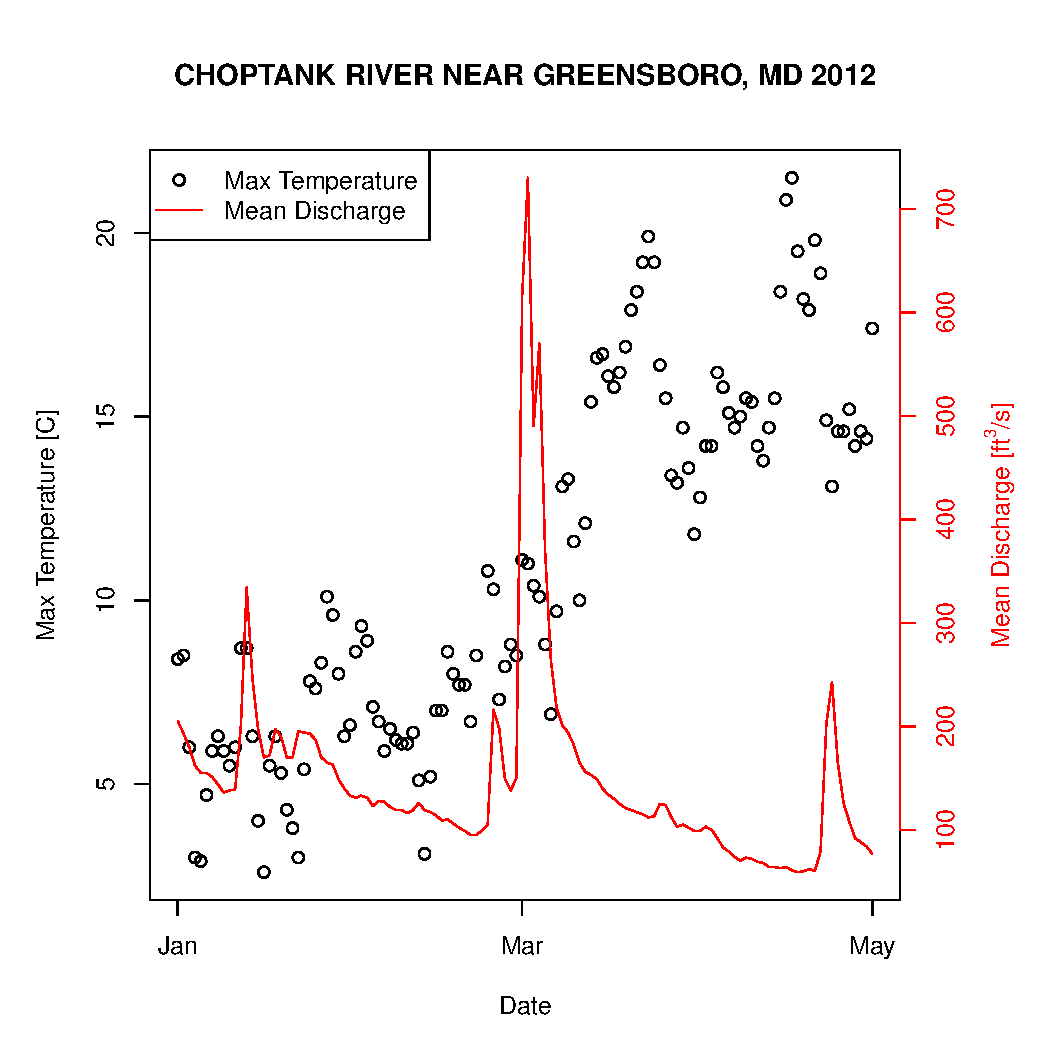
\includegraphics[width=1\linewidth,height=1\linewidth]{figure/getNWIStemperaturePlot} \caption[Temperature and discharge plot of Choptank River in 2012]{Temperature and discharge plot of Choptank River in 2012.\label{fig:getNWIStemperaturePlot}}
\end{figure}


\end{knitrout}



There are occasions where NWIS values are not reported as numbers, instead there might be text describing a certain event such as \texttt{"}Ice\texttt{"}.  Any value that cannot be converted to a number will be reported as NA in this package.

\FloatBarrier

%------------------------------------------------------------
\subsection{Unit Values}
\label{sec:usgsRT}
%------------------------------------------------------------
Any data that are collected at regular time intervals (such as 15-minute or hourly) are known as \texttt{"}Unit Values\texttt{"} - many of these are delivered on a real time basis and very recent data (even less than an hour old in many cases) are available through the function retrieveUnitNWISData.  Some of these Unit Values are available for the past several years, and some are only available for a recent time period such as 120 days or a year.  Here is an example of a retrieval of such data.  

\begin{knitrout}
\definecolor{shadecolor}{rgb}{0.969, 0.969, 0.969}\color{fgcolor}\begin{kframe}
\begin{alltt}

parameterCd <- \hlstring{"00060"}  # \hlfunctioncall{Discharge} (cfs)
startDate <- \hlstring{"2012-05-12"} 
endDate <- \hlstring{"2012-05-13"} 
dischargeToday <- \hlfunctioncall{retrieveUnitNWISData}(siteNumber, parameterCd, 
        startDate, endDate)
\end{alltt}
\end{kframe}
\end{knitrout}

Which produces the following dataframe:
\begin{knitrout}
\definecolor{shadecolor}{rgb}{0.969, 0.969, 0.969}\color{fgcolor}\begin{kframe}
\begin{verbatim}
  agency     site            dateTime X02_00060_00011
1   USGS 01491000 2012-05-12 00:00:00              83
2   USGS 01491000 2012-05-12 00:15:00              83
3   USGS 01491000 2012-05-12 00:30:00              83
4   USGS 01491000 2012-05-12 00:45:00              83
5   USGS 01491000 2012-05-12 01:00:00              85
6   USGS 01491000 2012-05-12 01:15:00              83
  X02_00060_00011_cd
1                  A
2                  A
3                  A
4                  A
5                  A
6                  A
\end{verbatim}
\end{kframe}
\end{knitrout}


Note that time now becomes important, so the variable datetime is a POSIXct, and the time zone is included in a separate column. Data is pulled from \url{http://waterservices.usgs.gov/rest/IV-Test-Tool.html}. There are occasions where NWIS values are not reported as numbers, instead a common example is \texttt{"}Ice\texttt{"}.  Any value that cannot be converted to a number will be reported as NA in this package.

\newpage


\FloatBarrier

%------------------------------------------------------------
\subsection{Water Quality Values}
\label{sec:usgsWQP}
%------------------------------------------------------------
To get USGS water quality data from water samples collected at the streamgage (as distinct from unit values collected through some type of automatic monitor) we can use the Water Quality Data Portal: \url{http://www.waterqualitydata.us/}. The raw data are obtained from the function  getRawQWData, with the similar input arguments: siteNumber, parameterCd, startDate, endDate, and interactive. The difference is in parameterCd, in this function multiple parameters can be queried using a vector, and setting parameterCd to \texttt{"}\texttt{"} will return all of the measured observations. The raw data can be overwelming (see Appendix \ref{sec:appendix2WQP}), a simplified version of the data can be obtained using getQWData.There is a large amount of data returned for each observation. 


\begin{knitrout}
\definecolor{shadecolor}{rgb}{0.969, 0.969, 0.969}\color{fgcolor}\begin{kframe}
\begin{alltt}
 
\hlcomment{# Dissolved Nitrate parameter codes:}
parameterCd <- \hlfunctioncall{c}(\hlstring{"00618"},\hlstring{"71851"})
startDate <- \hlstring{"1979-10-11"}
endDate <- \hlstring{"2012-12-18"}

dissolvedNitrate <- \hlfunctioncall{getRawQWData}(siteNumber, parameterCd, 
      startDate, endDate)

dissolvedNitrateSimple <- \hlfunctioncall{getQWData}(siteNumber, parameterCd, 
        startDate, endDate)
\hlfunctioncall{names}(dissolvedNitrateSimple)
\end{alltt}
\begin{verbatim}
[1] "dateTime"        "qualifier.71851" "value.71851"    
[4] "qualifier.00618" "value.00618"    
\end{verbatim}
\end{kframe}
\end{knitrout}

Note that in this dataframe, datetime is imported as Dates (no times are included), and the qualifier is either blank or \texttt{"}\verb@<@\texttt{"} signifying a censored value. A plotting example is shown in Figure \ref{fig:getQWtemperaturePlot}.

\begin{knitrout}
\definecolor{shadecolor}{rgb}{0.969, 0.969, 0.969}\color{fgcolor}\begin{kframe}
\begin{alltt}
\hlfunctioncall{with}(dissolvedNitrateSimple, \hlfunctioncall{plot}(
  dateTime, value.00618,
  xlab=\hlstring{"Date"},ylab = \hlfunctioncall{paste}(parameterINFO$srsname,
      \hlstring{"["},parameterINFO$parameter_units,\hlstring{"]"})
  ))
\hlfunctioncall{title}(ChoptankInfo$station.nm)
\end{alltt}
\end{kframe}\begin{figure}[]

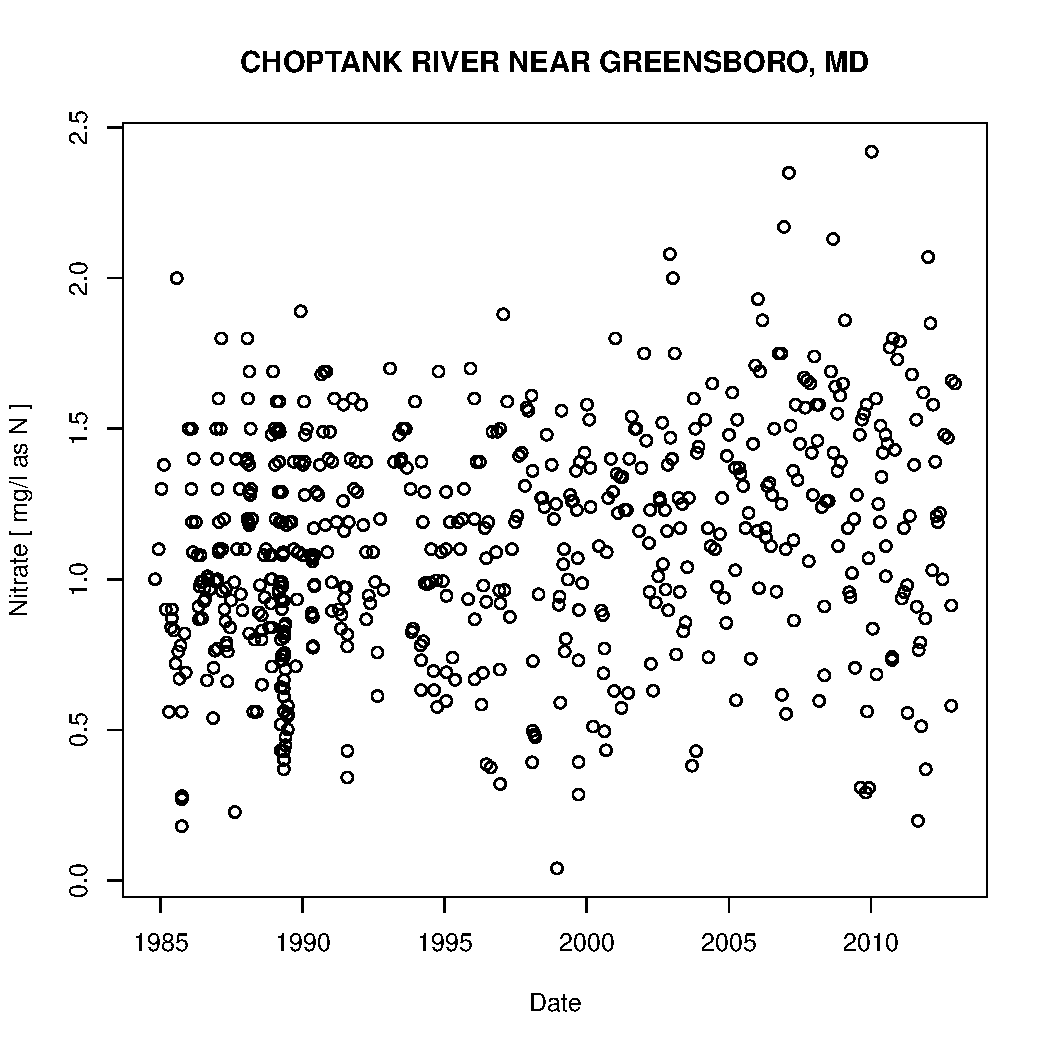
\includegraphics[width=\maxwidth]{figure/getQWtemperaturePlot} \caption[Nitrate plot of Choptank River]{Nitrate plot of Choptank River.\label{fig:getQWtemperaturePlot}}
\end{figure}


\end{knitrout}


\FloatBarrier

%------------------------------------------------------------
\subsection{STORET Water Quality Retrievals}
\label{sec:usgsSTORET}
%------------------------------------------------------------
There are additional data sets available on the Water Quality Data Portal (\url{http://www.waterqualitydata.us/}).  These data sets can be housed in either the STORET (data from EPA) or NWIS database.  Since STORET does not use USGS parameter codes, a \texttt{"}characteristic name\texttt{"} must be supplied.  The following example retrieves specific conductance from a DNR site in Wisconsin.

\begin{knitrout}
\definecolor{shadecolor}{rgb}{0.969, 0.969, 0.969}\color{fgcolor}\begin{kframe}
\begin{alltt}
specificCond <- \hlfunctioncall{getWQPData}(\hlstring{'WIDNR_WQX-10032762'}, 
        \hlstring{'Specific conductance'}, \hlstring{''}, \hlstring{''})
\hlfunctioncall{head}(specificCond)
\end{alltt}
\begin{verbatim}
    dateTime qualifier.Specific conductance
1 2011-02-14                               
2 2011-02-17                               
3 2011-03-03                               
4 2011-03-10                               
5 2011-03-29                               
6 2011-04-07                               
  value.Specific conductance
1                       1360
2                       1930
3                       1240
4                       1480
5                       1130
6                       1200
\end{verbatim}
\end{kframe}
\end{knitrout}


\FloatBarrier
%------------------------------------------------------------
\subsection{URL Construction}
\label{sec:usgsURL}
%------------------------------------------------------------
There may be times when you might be interested in seeing the URL (web address) that was used to obtain the raw data. The constructNWISURL function returns the URL.  Aside from input variables that have already been described, there is a new argument \texttt{"}service\texttt{"}. The service argument can be \texttt{"}dv\texttt{"} (daily values), \texttt{"}uv\texttt{"} (unit values), \texttt{"}qw\texttt{"} (NWIS water quality values), or \texttt{"}wqp\texttt{"} (general Water Quality Portal values).
 

\begin{knitrout}
\definecolor{shadecolor}{rgb}{0.969, 0.969, 0.969}\color{fgcolor}\begin{kframe}
\begin{alltt}
\hlcomment{# Dissolved Nitrate parameter codes:}
pCode <- \hlfunctioncall{c}(\hlstring{"00618"},\hlstring{"71851"})
startDate <- \hlstring{"1964-06-11"}
endDate <- \hlstring{"2012-12-18"}
url_qw <- \hlfunctioncall{constructNWISURL}(siteNumber,pCode,startDate,endDate,\hlstring{'qw'})
url_dv <- \hlfunctioncall{constructNWISURL}(siteNumber,\hlstring{"00060"},startDate,endDate,
                           \hlstring{'dv'},statCd=\hlstring{"00003"})
url_uv <- \hlfunctioncall{constructNWISURL}(siteNumber,\hlstring{"00060"},startDate,endDate,\hlstring{'uv'})
\end{alltt}
\end{kframe}
\end{knitrout}


\FloatBarrier

%------------------------------------------------------------
\section{Data Retrievals Structured For Use In The EGRET Package}
%------------------------------------------------------------ 
Rather than using the raw data as retrieved by the web, the dataRetrieval package also includes functions that return the data in a structure that has been designed to work with the EGRET R package (\url{https://github.com/USGS-R/EGRET/wiki}). In general, these dataframes may be much more 'R-friendly' than the raw data, and will contain additional date information that allows for efficient data analysis.

In this section, we use 3 dataRetrieval functions to get sufficient data to perform an EGRET analysis.  We will continue analyzing the Choptank River. We will be retrieving essentially the same data that were retrieved in the previous section, but in this case it will be structured into three EGRET-specific dataframes.  The daily discharge data will be placed in a dataframe called Daily.  The nitrate sample data will be placed in a dataframe called Sample.  The data about the site and the parameter will be placed in a dataframe called INFO.  Although these dataframes were designed to work with the EGRET R package, they can be very useful for a wide range of hydrologic studies that don't use EGRET.

%------------------------------------------------------------
\subsection{INFO Data}
%------------------------------------------------------------
The function to obtain metadata, or data about the streamgage and measured parameters is getMetaData. This function combines getSiteFileData and getParameterInfo, producing one dataframe called INFO.

\begin{knitrout}
\definecolor{shadecolor}{rgb}{0.969, 0.969, 0.969}\color{fgcolor}\begin{kframe}
\begin{alltt}
parameterCd <- \hlstring{"00618"}
INFO <-\hlfunctioncall{getMetaData}(siteNumber,parameterCd, interactive=FALSE)
\end{alltt}
\end{kframe}
\end{knitrout}


Column names in the INFO dataframe are listed in Appendix 2 (\ref{sec:appendix2INFO}).

\FloatBarrier

%------------------------------------------------------------
\subsection{Daily Data}
%------------------------------------------------------------
The function to obtain the daily values (discharge in this case) is getDVData.  It requires the inputs siteNumber, ParameterCd, StartDate, EndDate, interactive, and convert. Most of these arguments are described in the previous section, however \texttt{"}convert\texttt{"} is a new argument (defaults to TRUE), and it tells the program to convert the values from cubic feet per second (cfs) to cubic meters per second (cms). For EGRET applications with NWIS web retrieval, do not use this argument (the default is TRUE), EGRET assumes that discharge is always in cubic meters per second. If you don't want this conversion and are not using EGRET, set convert=FALSE in the function call. 

\begin{knitrout}
\definecolor{shadecolor}{rgb}{0.969, 0.969, 0.969}\color{fgcolor}\begin{kframe}
\begin{alltt}
siteNumber <- \hlstring{"01491000"}
startDate <- \hlstring{"2000-01-01"}
endDate <- \hlstring{"2013-01-01"}
\hlcomment{# This call will get NWIS (cfs) data , and convert it to cms:}
Daily <- \hlfunctioncall{getDVData}(siteNumber, \hlstring{"00060"}, startDate, endDate)
\end{alltt}
\begin{verbatim}
There are  4750 data points, and  4750 days.
\end{verbatim}
\end{kframe}
\end{knitrout}


Details of the Daily dataframe are listed below:

% latex table generated in R 3.0.1 by xtable 1.7-1 package
% Thu Aug 01 16:23:22 2013
\begin{table}[ht]
\centering
\begin{tabular}{rllll}
  \hline
 & ColumnName & Type & Description & Units \\ 
  \hline
1 & Date & Date & Date & date \\ 
  2 & Q & number & Discharge in cms & cms \\ 
  3 & Julian & number & Number of days since January 1, 1850 & days \\ 
  4 & Month & integer & Month of the year [1-12] & months \\ 
  5 & Day & integer & Day of the year [1-366] & days \\ 
  6 & DecYear & number & Decimal year & years \\ 
  7 & MonthSeq & integer & Number of months since January 1, 1850 & months \\ 
  8 & Qualifier & string & Qualifing code & character \\ 
  9 & i & integer & Index of days, starting with 1 & days \\ 
  10 & LogQ & number & Natural logarithm of Q & numeric \\ 
  11 & Q7 & number & 7 day running average of Q & cms \\ 
  12 & Q30 & number & 30 running average of Q & cms \\ 
   \hline
\end{tabular}
\caption{Daily dataframe} 
\end{table}




If there are discharge values of zero, the code will add a small constant to all of the daily discharges.  This constant is 0.001 times the mean discharge.  The code will also report on the number of zero and negative values and the size of the constant.  EGRET should only be used if the number of zero values is a very small fraction of the total days in the record (say less than 0.1\% of the days), and there are no negative discharge values.  Columns Q7 and Q30 are the 7 and 30 day running averages for the 7 or 30 days ending on this specific date.

\FloatBarrier

%------------------------------------------------------------
\subsection{Sample Data}
%------------------------------------------------------------
The function to obtain USGS sample data from the water quality portal is getSampleData. The arguments for this function are also siteNumber, ParameterCd, StartDate, EndDate, interactive. These are the same inputs as getRawQWData or getQWData as described in the previous section.

\begin{knitrout}
\definecolor{shadecolor}{rgb}{0.969, 0.969, 0.969}\color{fgcolor}\begin{kframe}
\begin{alltt}
parameterCd <- \hlstring{"00618"}
Sample <-\hlfunctioncall{getSampleData}(siteNumber,parameterCd,
      startDate, endDate)
\end{alltt}
\end{kframe}
\end{knitrout}


The function to obtain STORET sample data from the water quality portal is getSTORETSampleData. The arguments for this function are also siteNumber, ParameterCd, StartDate, EndDate, interactive. These are the same inputs as getRawQWData or getQWData as described in the previous section.

\begin{knitrout}
\definecolor{shadecolor}{rgb}{0.969, 0.969, 0.969}\color{fgcolor}\begin{kframe}
\begin{alltt}
site <- \hlstring{'WIDNR_WQX-10032762'}
characteristicName <- \hlstring{'Specific conductance'}
Sample <-\hlfunctioncall{getSTORETSampleData}(site,characteristicName,
      startDate, endDate)
\end{alltt}
\end{kframe}
\end{knitrout}



\pagebreak

Details of the Sample dataframe are listed below:

\begin{table}[!ht]
\begin{minipage}{\linewidth}
\begin{center}
\caption{Sample dataframe} 
\begin{tabular}{llll}
  \hline
ColumnName & Type & Description & Units \\ 
  \hline
Date & Date & Date & date \\ 
  ConcLow & number & Lower limit of concentration & mg/L \\ 
  ConcHigh & number & Upper limit of concentration & mg/L \\ 
  Uncen & integer & Uncensored data (1=true, 0=false) & integer \\ 
  ConcAve & number & Average of ConcLow and ConcHigh & mg/L \\ 
  Julian & number & Number of days since January 1, 1850 & days \\ 
  Month & integer & Month of the year [1-12] & months \\ 
  Day & integer & Day of the year [1-366] & days \\ 
  DecYear & number & Decimal year & years \\ 
  MonthSeq & integer & Number of months since January 1, 1850 & months \\ 
  SinDY & number & Sine of DecYear & numeric \\ 
  CosDY & number & Cosine of DecYear & numeric \\ 
  Q \footnotemark[1] & number & Discharge & cms \\ 
  LogQ \footnotemark[1] & number & Natural logarithm of discharge & numeric \\ 
   \hline
\end{tabular}
\end{center}
\end{minipage}
\end{table}

\footnotetext[1]{Discharge columns are populated from data in the Daily dataframe after calling the mergeReport function.}

\FloatBarrier


%------------------------------------------------------------
\subsection{Censored Values: Summation Explanation}
%------------------------------------------------------------
In the typical case where none of the data are censored (that is, no values are reported as \texttt{"}less-than\texttt{"} values) the ConcLow = ConcHigh = ConcAve all of which are equal to the reported value and Uncen=0.  In the typical form of censoring where a value is reported as less than the reporting limit, then ConcLow = NA, ConcHigh = reporting limit, ConcAve = 0.5 * reporting limit, and Uncen = 1.

As an example to understand how the dataRetrieval package handles a more complex censoring problem, let us say that in 2004 and earlier, we computed a total phosphorus (tp) as the sum of dissolved phosphorus (dp) and particulate phosphorus (pp). From 2005 and onward, we have direct measurements of total phosphorus (tp). A small subset of this fictional data looks like this:

\begin{center}

% latex table generated in R 3.0.1 by xtable 1.7-1 package
% Thu Aug 01 16:23:24 2013
\begin{table}[ht]
\centering
\begin{tabular}{rllrlrlr}
  \hline
 & cdate & rdp & dp & rpp & pp & rtp & tp \\ 
  \hline
1 & 2003-02-15 &  & 0.02 &  & 0.50 &  &  \\ 
  2 & 2003-06-30 & $<$ & 0.01 &  & 0.30 &  &  \\ 
  3 & 2004-09-15 & $<$ & 0.00 & $<$ & 0.20 &  &  \\ 
  4 & 2005-01-30 &  &  &  &  &  & 0.43 \\ 
  5 & 2005-05-30 &  &  &  &  & $<$ & 0.05 \\ 
  6 & 2005-10-30 &  &  &  &  & $<$ & 0.02 \\ 
   \hline
\end{tabular}
\caption{Example data} 
\end{table}



\end{center}


The dataRetrieval package will \texttt{"}add up\texttt{"} all the values in a given row to form the total for that sample. Thus, you only want to enter data that should be added together. For example, we might know the value for dp on 5/30/2005, but we don't want to put it in the table because under the rules of this data set, we are not suppose to add it in to the values in 2005.

For every sample, the EGRET package requires a pair of numbers to define an interval in which the true value lies (ConcLow and ConcHigh). In a simple non-censored case (the reported value is above the detection limit), ConcLow equals ConcHigh and the interval collapses down to a single point.In a simple censored case, the value might be reported as \verb@<@0.2, then ConcLow=NA and ConcHigh=0.2. We use NA instead of 0 as a way to elegantly handle future logarithm calculations.

For the more complex example case, let us say dp is reported as \verb@<@0.01 and pp is reported as 0.3. We know that the total must be at least 0.3 and could be as much as 0.31. Therefore, ConcLow=0.3 and ConcHigh=0.31. Another case would be if dp is reported as \verb@<@0.005 and pp is reported \verb@<@0.2. We know in this case that the true value could be as low as zero, but could be as high as 0.205. Therefore, in this case, ConcLow=NA and ConcHigh=0.205. The Sample dataframe for the example data is therefore:

\begin{knitrout}
\definecolor{shadecolor}{rgb}{0.969, 0.969, 0.969}\color{fgcolor}\begin{kframe}
\begin{verbatim}
        Date ConcLow ConcHigh Uncen ConcAve Julian Month
1 2003-02-15   0.520    0.520     1   0.520  55927     2
2 2003-06-30   0.310    0.310     1   0.310  56062     6
3 2004-09-15   0.205    0.205     1   0.205  56505     9
4 2005-01-30   0.430    0.430     1   0.430  56642     1
5 2005-05-30   0.050    0.050     1   0.050  56762     5
6 2005-10-30   0.020    0.020     1   0.020  56915    10
  Day DecYear MonthSeq    SinDY   CosDY
1  46    2003     1838  0.70407  0.7101
2 182    2003     1842  0.02575 -0.9997
3 259    2005     1857 -0.96251 -0.2712
4  30    2005     1861  0.48506  0.8745
5 151    2005     1865  0.52943 -0.8484
6 304    2006     1870 -0.87861  0.4775
\end{verbatim}
\end{kframe}
\end{knitrout}


\FloatBarrier

%------------------------------------------------------------ 
\subsection{User-Generated Data Files}
%------------------------------------------------------------ 
Aside from retrieving data from the USGS web services, the dataRetrieval package includes functions to generate the Daily and Sample data frame from local files.

%------------------------------------------------------------ 
\subsubsection{getDailyDataFromFile}
%------------------------------------------------------------ 
getDailyDataFromFile will load a user-supplied text file and convert it to the Daily dataframe. The file should have two columns, the first dates, the second values.  The dates should be formatted either mm/dd/yyyy or yyyy-mm-dd. Using a 4-digit year is required. This function has the following inputs: filePath, fileName,hasHeader (TRUE/FALSE), separator, qUnit, and interactive (TRUE/FALSE). filePath is a string that defines the path to your file. This can either be a full path, or path relative to your R working directory. The input fileName is a string that defines the file name (including the extension).

Text files that contain this sort of data require some sort of a separator, for example, a 'csv' file (comma-separated value) file uses a comma to separate the date and value column. A tab delimited file would use a tab (\texttt{"}\verb@\t@\texttt{"}) rather than the comma (\texttt{"},\texttt{"}). The type of separator you use can be defined in the function call in the \texttt{"}separator\texttt{"} argument, the default is \texttt{"},\texttt{\texttt{"}}. Another function input is a logical variable: hasHeader.  The default is TRUE. If your data does not have column names, set this variable to FALSE.

Finally, qUnit is a numeric argument that defines the discharge units used in the input file.  The default is qUnit = 1 which assumes discharge is in cubic feet per second.  If the discharge in the file is already in cubic meters per second then set qUnit = 2.  If it is in some other units (like liters per second or acre-feet per day), the user will have to pre-process the data with a unit conversion that changes it to either cubic feet per second or cubic meters per second.

So, if you have a file called \texttt{"}ChoptankRiverFlow.txt\texttt{"} located in a folder called \texttt{"}RData\texttt{"} on the C drive (this is a Window's example), and the file is structured as follows (tab-separated):
\begin{verbatim}
date  Qdaily
10/1/1999  107
10/2/1999  85
10/3/1999	76
10/4/1999	76
10/5/1999	113
10/6/1999	98
...
\end{verbatim}

The call to open this file, convert the discharge to cubic meters per second, and populate the Daily data frame would be:
\begin{knitrout}
\definecolor{shadecolor}{rgb}{0.969, 0.969, 0.969}\color{fgcolor}\begin{kframe}
\begin{alltt}
fileName <- \hlstring{"ChoptankRiverFlow.txt"}
filePath <-  \hlstring{"C:/RData/"}
Daily <- \hlfunctioncall{getDailyDataFromFile}(filePath,fileName,
                    separator=\hlstring{"\textbackslash{}t"})
\end{alltt}
\end{kframe}
\end{knitrout}


\FloatBarrier

%------------------------------------------------------------ 
\subsubsection{getSampleDataFromFile}
%------------------------------------------------------------ 
Similarly to the previous section, getSampleDataFromFile will import a user-generated file and populate the Sample dataframe. The difference between sample data and discharge data is that the code requires a third column that contains a remark code, either blank or \texttt{"}\verb@<@\texttt{"}, which will tell the program that the data was 'left-censored' (or, below the detection limit of the sensor). Therefore, the data is required to be in the form: date, remark, value.  If multiple constituents are going to be summed, the format can be date, remark\_A, value\_A, remark\_b, value\_b, etc... An example of a comma-delimited file would be:

\begin{verbatim}
cdate;remarkCode;Nitrate
10/7/1999,,1.4
11/4/1999,<,0.99
12/3/1999,,1.42
1/4/2000,,1.59
2/3/2000,,1.54
...
\end{verbatim}
The call to open this file, and populate the Sample dataframe would be:
\begin{knitrout}
\definecolor{shadecolor}{rgb}{0.969, 0.969, 0.969}\color{fgcolor}\begin{kframe}
\begin{alltt}
fileName <- \hlstring{"ChoptankRiverNitrate.csv"}
filePath <-  \hlstring{"C:/RData/"}
Sample <- \hlfunctioncall{getSampleDataFromFile}(filePath,fileName,
                                separator=\hlstring{","})
\end{alltt}
\end{kframe}
\end{knitrout}


\FloatBarrier

%------------------------------------------------------------
\subsection{Merge Report}
%------------------------------------------------------------
Finally, there is a function called mergeReport that will look at both the Daily and Sample dataframe, and populate Q and LogQ columns into the Sample dataframe. The default arguments are Daily and Sample, however if you want to use other similarly structured dataframes, you can specify localDaily or localSample. Once mergeReport has been run, the Sample dataframe will be augumented with the daily discharges for all the days with samples.  None of the water quality functions in EGRET will work without first having run the mergeReport function.


\begin{knitrout}
\definecolor{shadecolor}{rgb}{0.969, 0.969, 0.969}\color{fgcolor}\begin{kframe}
\begin{alltt}
siteNumber <- \hlstring{"01491000"}
parameterCd <- \hlstring{"00631"}  # Nitrate
startDate <- \hlstring{"2000-01-01"}
endDate <- \hlstring{"2013-01-01"}

Daily <- \hlfunctioncall{getDVData}(siteNumber, \hlstring{"00060"}, startDate, endDate)
\end{alltt}
\begin{verbatim}
There are  4750 data points, and  4750 days.
\end{verbatim}
\begin{alltt}
Sample <- \hlfunctioncall{getSampleData}(siteNumber,parameterCd, startDate, endDate)
Sample <- \hlfunctioncall{mergeReport}()
\end{alltt}
\begin{verbatim}

 Discharge Record is 4750 days long, which is 13 years
 First day of the discharge record is 2000-01-01 and last day is 2013-01-01
 The water quality record has 220 samples
 The first sample is from 2000-01-04 and the last sample is from 2012-12-18
 Discharge: Minimum, mean and maximum 0.00991 4.55 246
 Concentration: Minimum, mean and maximum 0.2 1.3 2.4
 Percentage of the sample values that are censored is 0 %
\end{verbatim}
\begin{alltt}
\hlfunctioncall{head}(Sample)
\end{alltt}
\begin{verbatim}
        Date ConcLow ConcHigh Uncen ConcAve Julian Month
1 2000-01-04    1.59     1.59     1    1.59  54789     1
2 2000-02-03    1.54     1.54     1    1.54  54819     2
3 2000-02-15    1.37     1.37     1    1.37  54831     2
4 2000-02-19    1.24     1.24     1    1.24  54835     2
5 2000-03-23    0.52     0.52     1    0.52  54868     3
6 2000-06-05    1.11     1.11     1    1.11  54942     6
  Day DecYear MonthSeq   SinDY   CosDY      Q   LogQ
1   4    2000     1801 0.06005  0.9982  2.747 1.0104
2  34    2000     1802 0.54392  0.8391  3.936 1.3702
3  46    2000     1802 0.70407  0.7101 10.845 2.3837
4  50    2000     1802 0.75113  0.6602 15.518 2.7420
5  83    2000     1803 0.98809  0.1539 56.917 4.0416
6 157    2000     1806 0.43940 -0.8983  1.812 0.5946
\end{verbatim}
\end{kframe}
\end{knitrout}


\FloatBarrier

%------------------------------------------------------------
\subsection{EGRET Plots}
%------------------------------------------------------------
As has been mentioned, the data is specifically formatted to be used with the EGRET package. The EGRET package has powerful modeling capabilities using WRTDS, but also has a variety of graphing and tablular tools to explore the data without using the WRTDS algorithm. See the EGRET vignette, user guide, and/or wiki (\url{https://github.com/USGS-R/EGRET/wiki}) for detailed information. The following figure is an example of one of the plotting functions that can be used directly from the dataRetrieval dataframes.

\begin{knitrout}
\definecolor{shadecolor}{rgb}{0.969, 0.969, 0.969}\color{fgcolor}\begin{kframe}
\begin{alltt}
\hlcomment{# Continuing Choptank example from the previous sections}
\hlfunctioncall{library}(EGRET)
\hlfunctioncall{multiPlotDataOverview}()
\end{alltt}
\end{kframe}\begin{figure}[]

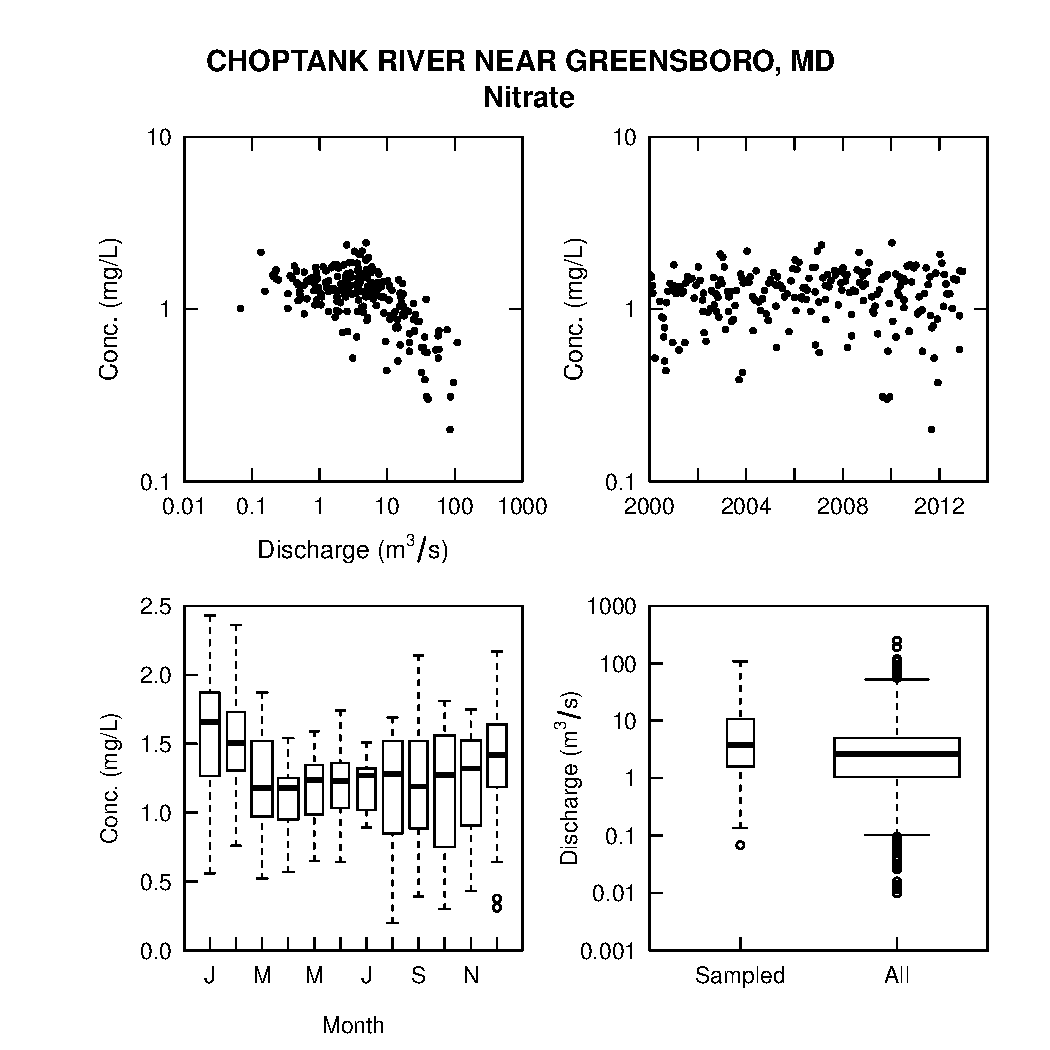
\includegraphics[width=\maxwidth]{figure/egretEx} \caption[Default multiPlotDataOverview]{Default multiPlotDataOverview\label{fig:egretEx}}
\end{figure}


\end{knitrout}


\clearpage
\appendix

%------------------------------------------------------------ 
\section{Getting Started in R}
\label{sec:appendix1}
%------------------------------------------------------------ 
This section describes the options for downloading and installing the dataRetrieval package.

%------------------------------------------------------------
\subsection{New to R?}
%------------------------------------------------------------ 
If you are new to R, you will need to first install the latest version of R, which can be found here: \url{http://www.r-project.org/}.

There are many options for running and editing R code, one nice environment to learn R is RStudio. RStudio can be downloaded here: \url{http://rstudio.org/}. Once R and RStudio are installed, the dataRetrieval package needs to be installed as described in the next section.

At any time, you can get information about any function in R by typing a question mark before the functions name.  This will open a file (in RStudio, in the Help window) that describes the function, the required arguments, and provides working examples.

\begin{knitrout}
\definecolor{shadecolor}{rgb}{0.969, 0.969, 0.969}\color{fgcolor}\begin{kframe}
\begin{alltt}
?removeDuplicates
\end{alltt}
\end{kframe}
\end{knitrout}


To see the raw code for a particular code, type the name of the function:
\begin{knitrout}
\definecolor{shadecolor}{rgb}{0.969, 0.969, 0.969}\color{fgcolor}\begin{kframe}
\begin{alltt}
removeDuplicates
\end{alltt}
\begin{verbatim}
function(localSample=Sample) {  
  Sample1 <- localSample[!duplicated(localSample[c("DecYear","ConcHigh")]),]
  
  return(Sample1)
}
<environment: namespace:dataRetrieval>
\end{verbatim}
\end{kframe}
\end{knitrout}


%------------------------------------------------------------
\subsection{R User: Installing dataRetrieval}
%------------------------------------------------------------ 
Before installing dataRetrieval, the zoo packages must be installed from CRAN:

\begin{knitrout}
\definecolor{shadecolor}{rgb}{0.969, 0.969, 0.969}\color{fgcolor}\begin{kframe}
\begin{alltt}
\hlfunctioncall{install.packages}(\hlstring{"zoo"})
\hlfunctioncall{install.packages}(\hlstring{"dataRetrieval"}, repos=\hlstring{"http://usgs-r.github.com"}, type=\hlstring{"source"})
\end{alltt}
\end{kframe}
\end{knitrout}


It is a good idea to re-start R after installing the package, especially if installing an updated version. Some users have found it necessary to delete the previous version's package folder before installing newer version of dataRetrieval. If you are experiencing issues after updating a package, trying deleting the package folder - the default location for Windows is something like this: C:/Users/userA/Documents/R/win-library/2.15/dataRetrieval, and the default for a Mac: /Users/userA/Library/R/2.15/library/dataRetrieval. Then, re-install the package using the directions above. Moving to CRAN should solve this problem.

After installing the package, you need to open the library each time you re-start R.  This is done with the simple command:
\begin{knitrout}
\definecolor{shadecolor}{rgb}{0.969, 0.969, 0.969}\color{fgcolor}\begin{kframe}
\begin{alltt}
\hlfunctioncall{library}(dataRetrieval)
\end{alltt}
\end{kframe}
\end{knitrout}


%------------------------------------------------------------ 
\section{Columns Names}
\label{sec:appendix2}
%------------------------------------------------------------ 

%------------------------------------------------------------
\subsection{INFO dataframe}
\label{sec:appendix2INFO}
%------------------------------------------------------------

% latex table generated in R 3.0.1 by xtable 1.7-1 package
% Thu Aug 01 16:23:26 2013
\begin{table}[ht]
\centering
\begin{tabular}{rl}
  \hline
 & ColumnNames \\ 
  \hline
1 & agency.cd \\ 
  2 & site.no \\ 
  3 & station.nm \\ 
  4 & site.tp.cd \\ 
  5 & lat.va \\ 
  6 & long.va \\ 
  7 & dec.lat.va \\ 
  8 & dec.long.va \\ 
  9 & coord.meth.cd \\ 
  10 & coord.acy.cd \\ 
  11 & coord.datum.cd \\ 
  12 & dec.coord.datum.cd \\ 
  13 & district.cd \\ 
  14 & state.cd \\ 
  15 & county.cd \\ 
  16 & country.cd \\ 
  17 & map.nm \\ 
  18 & map.scale.fc \\ 
  19 & alt.va \\ 
  20 & alt.meth.cd \\ 
  21 & alt.acy.va \\ 
  22 & alt.datum.cd \\ 
  23 & huc.cd \\ 
  24 & basin.cd \\ 
  25 & topo.cd \\ 
  26 & construction.dt \\ 
  27 & inventory.dt \\ 
  28 & drain.area.va \\ 
  29 & contrib.drain.area.va \\ 
  30 & tz.cd \\ 
  31 & local.time.fg \\ 
  32 & reliability.cd \\ 
  33 & project.no \\ 
  34 & queryTime \\ 
  35 & drainSqKm \\ 
  36 & shortName \\ 
  37 & staAbbrev \\ 
  38 & param.nm \\ 
  39 & param.units \\ 
  40 & paramShortName \\ 
  41 & paramNumber \\ 
  42 & constitAbbrev \\ 
   \hline
\end{tabular}
\caption{Column names in the INFO dataframe} 
\end{table}



\FloatBarrier

%------------------------------------------------------------
\subsection{Water Quality Portal}
\label{sec:appendix2WQP}
%------------------------------------------------------------

There are 62 columns returned from the water quality portal. 

% latex table generated in R 3.0.1 by xtable 1.7-1 package
% Thu Aug 01 16:23:26 2013
\begin{table}[ht]
\centering
\begin{tabular}{rl}
  \hline
 & ColumnNames \\ 
  \hline
1 & OrganizationIdentifier \\ 
  2 & OrganizationFormalName \\ 
  3 & ActivityIdentifier \\ 
  4 & ActivityTypeCode \\ 
  5 & ActivityMediaName \\ 
  6 & ActivityMediaSubdivisionName \\ 
  7 & ActivityStartDate \\ 
  8 & ActivityStartTime.Time \\ 
  9 & ActivityStartTime.TimeZoneCode \\ 
  10 & ActivityEndDate \\ 
  11 & ActivityEndTime.Time \\ 
  12 & ActivityEndTime.TimeZoneCode \\ 
  13 & ActivityDepthHeightMeasure.MeasureValue \\ 
  14 & ActivityDepthHeightMeasure.MeasureUnitCode \\ 
  15 & ActivityDepthAltitudeReferencePointText \\ 
  16 & ActivityTopDepthHeightMeasure.MeasureValue \\ 
  17 & ActivityTopDepthHeightMeasure.MeasureUnitCode \\ 
  18 & ActivityBottomDepthHeightMeasure.MeasureValue \\ 
  19 & ActivityBottomDepthHeightMeasure.MeasureUnitCode \\ 
  20 & ProjectIdentifier \\ 
  21 & ActivityConductingOrganizationText \\ 
  22 & MonitoringLocationIdentifier \\ 
  23 & ActivityCommentText \\ 
  24 & SampleAquifer \\ 
  25 & HydrologicCondition \\ 
  26 & HydrologicEvent \\ 
  27 & SampleCollectionMethod.MethodIdentifier \\ 
  28 & SampleCollectionMethod.MethodIdentifierContext \\ 
  29 & SampleCollectionMethod.MethodName \\ 
  30 & SampleCollectionEquipmentName \\ 
  31 & ResultDetectionConditionText \\ 
  32 & CharacteristicName \\ 
  33 & ResultSampleFractionText \\ 
  34 & ResultMeasureValue \\ 
  35 & ResultMeasure.MeasureUnitCode \\ 
  36 & MeasureQualifierCode \\ 
  37 & ResultStatusIdentifier \\ 
  38 & StatisticalBaseCode \\ 
  39 & ResultValueTypeName \\ 
  40 & ResultWeightBasisText \\ 
   \hline
\end{tabular}
\caption{Column names in dissolvedNitrate} 
\end{table}



\FloatBarrier

% latex table generated in R 3.0.1 by xtable 1.7-1 package
% Thu Aug 01 16:23:26 2013
\begin{table}[ht]
\centering
\begin{tabular}{rl}
  \hline
 & ColumnNames\_Continued \\ 
  \hline
1 & ResultTimeBasisText \\ 
  2 & ResultTemperatureBasisText \\ 
  3 & ResultParticleSizeBasisText \\ 
  4 & PrecisionValue \\ 
  5 & ResultCommentText \\ 
  6 & USGSPCode \\ 
  7 & ResultDepthHeightMeasure.MeasureValue \\ 
  8 & ResultDepthHeightMeasure.MeasureUnitCode \\ 
  9 & ResultDepthAltitudeReferencePointText \\ 
  10 & SubjectTaxonomicName \\ 
  11 & SampleTissueAnatomyName \\ 
  12 & ResultAnalyticalMethod.MethodIdentifier \\ 
  13 & ResultAnalyticalMethod.MethodIdentifierContext \\ 
  14 & ResultAnalyticalMethod.MethodName \\ 
  15 & MethodDescriptionText \\ 
  16 & LaboratoryName \\ 
  17 & AnalysisStartDate \\ 
  18 & ResultLaboratoryCommentText \\ 
  19 & DetectionQuantitationLimitTypeName \\ 
  20 & DetectionQuantitationLimitMeasure.MeasureValue \\ 
  21 & DetectionQuantitationLimitMeasure.MeasureUnitCode \\ 
  22 & PreparationStartDate \\ 
   \hline
\end{tabular}
\caption{Column names in dissolvedNitrate} 
\end{table}



\clearpage

%------------------------------------------------------------ 
\section{Creating tables in Microsoft from R}
\label{app:createWordTable}
%------------------------------------------------------------
There are a few steps that are required in order to create a table in a Microsoft product (Excel, Word, Powerpoint, etc.) from an R dataframe. There are certainly a variety of good methods, one of which is detailed here. The example we will step through here will be to create a table in Microsoft Word based on the dataframe tableData:

\begin{knitrout}
\definecolor{shadecolor}{rgb}{0.969, 0.969, 0.969}\color{fgcolor}\begin{kframe}
\begin{alltt}
availableData <- \hlfunctioncall{getDataAvailability}(siteNumber)
dailyData <- availableData[\hlstring{"dv"} == availableData$service,]
dailyData <- dailyData[\hlstring{"00003"} == dailyData$statCd,]

tableData <- \hlfunctioncall{with}(dailyData, 
      \hlfunctioncall{data.frame}(
        shortName=srsname, 
        Start=startDate, 
        End=endDate, 
        Count=count,
        Units=parameter_units)
      )
tableData
\end{alltt}
\begin{verbatim}
                               shortName      Start
1                     Temperature, water 2010-10-01
2               Stream flow, mean. daily 1948-01-01
3                   Specific conductance 2010-10-01
4 Suspended sediment concentration (SSC) 1980-10-01
5           Suspended sediment discharge 1980-10-01
         End Count      Units
1 2012-05-09   529      deg C
2 2013-07-31 23954        cfs
3 2012-05-09   527 uS/cm @25C
4 1991-09-30  3651       mg/l
5 1991-09-30  3652   tons/day
\end{verbatim}
\end{kframe}
\end{knitrout}


First, save the dataframe as a tab delimited file (you don't want to use comma delimited because there are commas in some of the data elements):


\begin{knitrout}
\definecolor{shadecolor}{rgb}{0.969, 0.969, 0.969}\color{fgcolor}\begin{kframe}
\begin{alltt}
\hlfunctioncall{write.table}(tableData, file=\hlstring{"tableData.tsv"},sep=\hlstring{"\textbackslash{}t"},
            row.names = FALSE,quote=FALSE)
\end{alltt}
\end{kframe}
\end{knitrout}


This will save a file in your working directory called tableData.tsv.  You can see your working directory by typing getwd() in the R console. Opening the file in a general-purpose text editor, you should see the following:

\begin{verbatim}
shortName  Start  End	Count	Units
Temperature, water	2010-10-01	2012-06-24	575	deg C
Stream flow, mean. daily	1948-01-01	2013-03-13	23814	cfs
Specific conductance	2010-10-01	2012-06-24	551	uS/cm @25C
Suspended sediment concentration (SSC)	1980-10-01	1991-09-30	3651	mg/l
Suspended sediment discharge	1980-10-01	1991-09-30	3652	tons/day
\end{verbatim}

To open this file in Excel:
\begin{enumerate}
\item Open Excel
\item Click on the File tab
\item Click on the Open option
\item Browse to the working directory (as shown in the results of getwd())
\item Next to the File name text box, change the dropdown type to All Files (*.*)
\item Double click tableData.tsv
\item A text import wizard will open up, in the first window, choose the Delimited radio button if it is not automatically picked, then click on Next.
\item In the second window, click on the Tab delimiter if it is not automatically checked, then click Finished.
\item Use the many formatting tools within Excel to customize the table
\end{enumerate}

From Excel, it is simple to copy and paste the tables in other Microsoft products. An example using one of the default Excel table formats is here.

\begin{figure}[ht!]
\centering
 \resizebox{0.9\textwidth}{!}{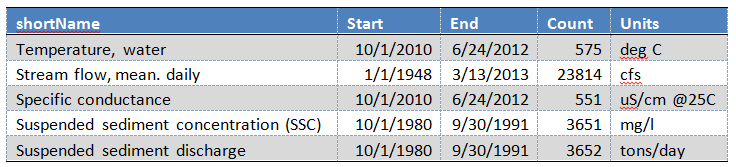
\includegraphics{table1.png}} 
\caption{A simple table produced in Microsoft Excel}
\label{overflow}
\end{figure}

\clearpage

%------------------------------------------------------------
% BIBLIO
%------------------------------------------------------------
\begin{thebibliography}{10}

\bibitem{HirschI}
Helsel, D.R. and R. M. Hirsch, 2002. Statistical Methods in Water Resources Techniques of Water Resources Investigations, Book 4, chapter A3. U.S. Geological Survey. 522 pages. \url{http://pubs.usgs.gov/twri/twri4a3/}

\bibitem{HirschII}
Hirsch, R. M., Moyer, D. L. and Archfield, S. A. (2010), Weighted Regressions on Time, Discharge, and Season (WRTDS), with an Application to Chesapeake Bay River Inputs. JAWRA Journal of the American Water Resources Association, 46: 857-880. doi: 10.1111/j.1752-1688.2010.00482.x \url{http://onlinelibrary.wiley.com/doi/10.1111/j.1752-1688.2010.00482.x/full}

\bibitem{HirschIII}
Sprague, L. A., Hirsch, R. M., and Aulenbach, B. T. (2011), Nitrate in the Mississippi River and Its Tributaries, 1980 to 2008: Are We Making Progress? Environmental Science \& Technology, 45 (17): 7209-7216. doi: 10.1021/es201221s \url{http://pubs.acs.org/doi/abs/10.1021/es201221s}

\end{thebibliography}

\end{document}

\end{document}
